\documentclass[UTF8]{ctexart}
\usepackage{amsmath,amssymb,amsfonts}
\usepackage{graphicx}%插入图片的宏包。
\usepackage{pythonhighlight}
\usepackage{tikz}%画图功能宏包
\title{有限差分求解抛物方程}
\author{向涛:~202021001395}
\date{\today}
\usepackage{geometry}
\geometry{left=1.25in,right=1.25in,top=1in,bottom=1in}
\usepackage{fancyhdr}
\pagestyle{fancy} 
\fancyhf{}
\fancyhead[L]{\bfseries\thepage}                                                           
\begin{document}
\maketitle
\section{模型问题}
\begin{equation}
\left \{
\begin{aligned}
& \dfrac{\partial u}{\partial t}-k\dfrac{\partial^2 u}{\partial x^2}=0 \\
& u(0,t)=0,~~u(1,t)=0,~~t\in [0,0.1] \\
& u(x,0) = e^{-\dfrac{(x-0.25)^2}{0.01}}+0.1*sin(20\pi x), x\in (0,1)
\end{aligned}
\right.
\end{equation}

其中系数$k=1$.请用向后差分法求解.

\section{空间离散和时间离散}

向后差分格式是一种隐式的求解格式,需要求解线性方程组.在求解方程前我们需要对求解的区域进行网格剖分,取空间步长和时间步长分别为$h=\dfrac{I}{N},\tau= \dfrac{T}{M}$,对空间变量$x$所属的区间$[0,I]$和时间变量$t$所属的区间$[0,T]$做如下均匀剖分:

\begin{equation}
0=x_0<x_1<\cdots<x_N=I,~0=t_0<t_1<\cdots<t_M=T
\end{equation}

其中$x_i = ih,t_k=K\tau~~i=0,1,\cdots,N~~K=0,1,\cdots,M$.

用两族平行直线$x=x_j(0,1,\cdots,N)$和$t=t_k(k=0,1,\cdots,M)$将求解区域分割为网格形式,对网格的节点集合我们用如下的记号表示,在二维我们一般用$\Omega$与$\partial\Omega$,在这里我用$\overline{G}$表示整个网格节点,$G_h,\Gamma_h$分别表示网格内部节点和边界节点,用集合来表示就是:



\begin{equation}
\left \{
\begin{aligned}
& \overline{G}=G_h \cup \Gamma_h=\{ (x_j,t_k):0\leq j\leq N;0\leq k \leq M \} \\
& G_h = \{ (x_j,t_k):0<j<N;0<k\leq M \} \\
& \Gamma_h=\{ (x_j,t_k):j=0,N;k=1,\cdots,M \} \cup \{  (x_j,t_0):j=0,\cdots,N \}
\end{aligned}
\right.
\end{equation}

下图显示的是网格剖分的形式,假设空间轴在横轴,时间轴在竖轴.

\begin{center}
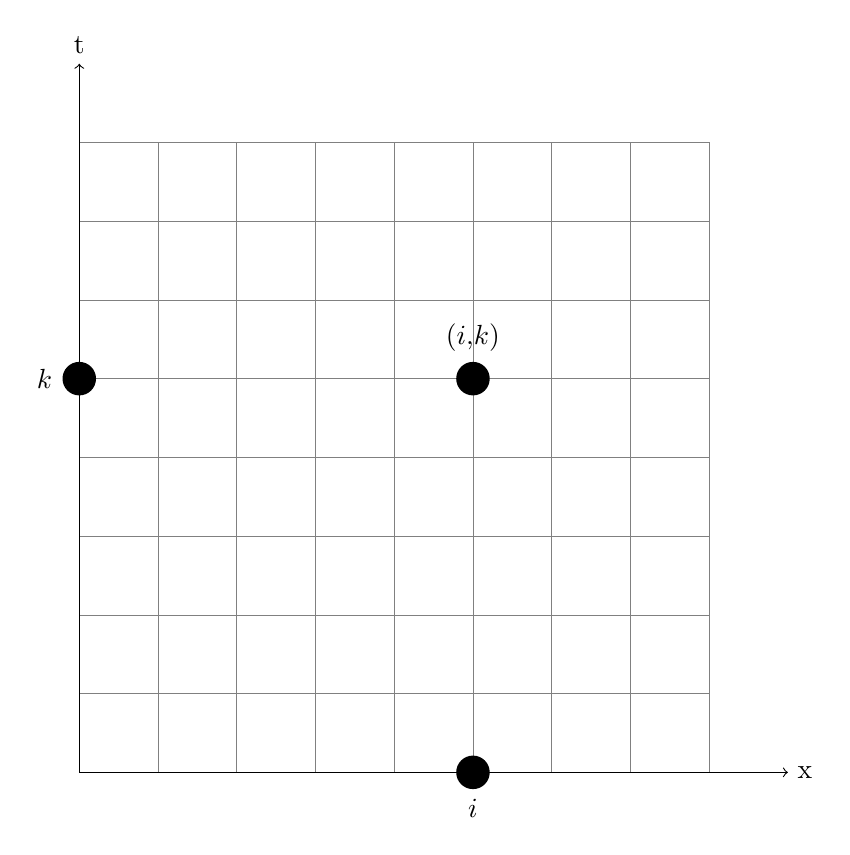
\begin{tikzpicture}
\draw[help lines,step=1]
(0,0) grid (8,8);
\node [circle,fill=black,inner sep=2pt,label=above:$(i\text{,}k)$] (A) at(5,5){$o$};
\node [circle,fill=black,inner sep=2pt,label=left:$k$] (A) at(0,5){$o$};
\node [circle,fill=black,inner sep=2pt,label=below:$i$] (A) at(5,0){$o$};
\draw[->](0,0)--(9,0) node[right]{x};
\draw[->](0,0)--(0,9) node[above]{t};
\end{tikzpicture}
\end{center}

为了描述方便用$u_j^k$表示差分解在网格节点$(x_j,t_k)$处的分量,下面将采用逐层计算的思想建立向后差分格式,根据已知的边界条件可知,在时间轴的两端边界点的值是已知的(也就是网格边界对应的两条竖线),在空间轴的底层也就是第0层是已知的(也就是x轴),那么我们的目的就是通过已知的第0层来计算第1层的数据,同时不考虑边界点,因为边界点是已知的,因此只需要计算内部节点的数据,注意到顶层的数据并不是边界点,因此还要计算顶层的数据,下面开始介绍一维情形下向后差分格式的具体思路.

因为第0层数据已经知道,便可以计算第1层的数据,假设现在已经计算到了第$k$层,需要计算第$(k+1)$层(简称当前层),考虑当前层上的任意内节点$(x_j,t_{k+1})$,规定其差分格式可用的模板点为

\begin{center}
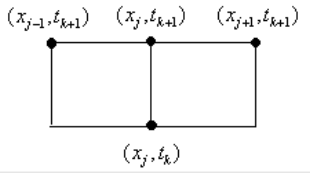
\includegraphics[scale= 0.6]{1.png}
\end{center}

对$(x_j,t_k)$处的微分方程

\begin{equation}
\dfrac{\partial u}{\partial t}=\dfrac{\partial^2 u}{\partial x^2}
\end{equation}

离散化,通常的方法是Taylor展式,不仅可以离散微分方程变成差分方程,还能够得到截断误差的阶,但是我们这里为了方便采用差商逼近导数的方法,则有

\begin{equation}
\dfrac{\partial u(x_j,t_{k+1})}{\partial t}\approx\dfrac{u(x_j,t_{k+1})-u(x_j,t_k)}{\tau}
\end{equation}

\begin{equation}
\dfrac{\partial^2u(x_j,t_{k+1})}{\partial x^2}\approx \dfrac{u(x_{j+1},t_{k+1})-2u(x_j,t_{k+1})+u(x_{j-1},t_{k+1})}{h^2}
\end{equation}

结合$(4)~(5)~(6)$式,并舍掉相关的误差,便可以得到向后差分格式

\begin{equation}
\dfrac{u_j^{k+1}-u_j^k}{\tau} = \dfrac{u_{j+1}^{k+1}-2u_j^{k+1}+u_{j-1}^{k+1}}{h^2}
\end{equation}

对$(7)$式两边同时乘以$\tau$,然后可以化简成如下的形式

\begin{equation}
-ru_{j-1}^{k+1}+(1+2r)u_j^{k+1}-ru_{j+1}^{k+1}=u_j^k
\end{equation}

其中$r=\dfrac{\tau}{h^2}$称为网格比,将$(8)$式写成矩阵形式就是

\begin{equation}
AU^{k+1}=U^k
\end{equation}

其中$A$的形式为

\[
\mathbf{A}=\left [ 
\begin{array}{ccccc}
1+2r & -r &  &  & \\
-r & 1+2r & -r &  & \\
   & \ddots & \ddots & \ddots & \\
 &  & -r & 1+2r & -r \\
 &  &  &-r  &1+2r 
\end{array}
 \right]
\]

\section{线性方程组的求解}

经过第二步的处理,抛物方程的解对应为线性方程组$(9)$的解,如果从数学理论分析的角度区求解,比如用克拉默法则,这无疑是一个巨大的工程,时间复杂度极其的高,如果通过对矩阵$A$求逆矩阵也是非常困难的,因为我们分隔的节点很多,那么矩阵$A$的维度会非常的大,此时求逆非常的困难,所以我们需要用迭代的方法求解$(9)$,在时间复杂度和空间复杂度上都会带来很大的好处.

一般来说线性方程组的迭代法有很多,比如Jacobi,Gauss-seidel,SOR,SSOR等,这里我采用的是Jacobi迭代方法求解线性方程组,具体的思路就是考虑分裂A=D-L-U,其中D是A的对角线部分,-L和-U分别为A的严格下三角和严格上三角部分,即可得Jacobi迭代方法:
\begin{equation}
x^{(k+1)} = D^{-1}(L+U)x_{(k)}+D^{-1}b,~k=1,2,\cdots,n.
\end{equation}
对应迭代矩阵为
\begin{equation}
G_{J}=(D)^{-1}(L+U).
\end{equation}

即可得到分量形式
\begin{equation}
x^{(k+1)}_i = \frac{1}{a_{ii}}\left(b_i-\sum^{n}_{j=1,j\neq i}a_{ij}x^{(k)}_j ,i=1,2,\cdots,n. \right)
\end{equation}

然后利用计算机进行编程求解.求解的结果如下图1(代码见附录):\footnote{本次实验报告的代码编程语言为:python,版本:3.8.6,IDE是pytharm 20.3.3 for linux,操作系统基于linux-ubuntu20.10}

\begin{figure}
    \centering
    \begin{minipage}{0.48\linewidth}
    \centering
         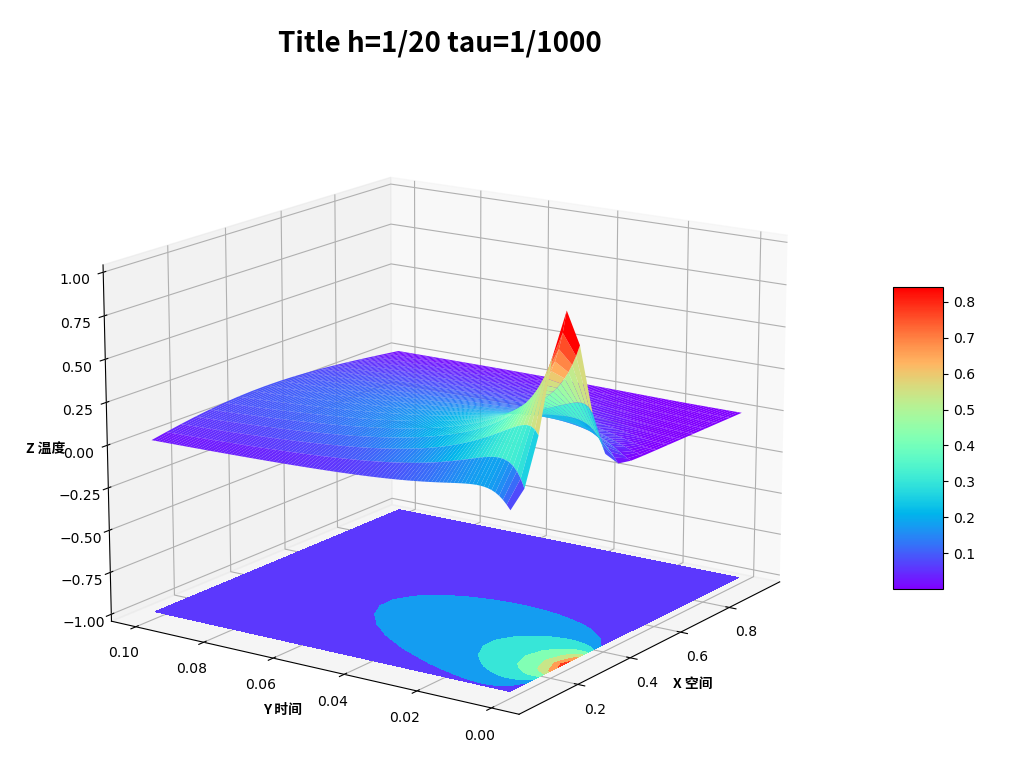
\includegraphics[scale= 0.2]{2.png}
    \end{minipage}
    \begin{minipage}{0.48\linewidth}
    \centering
         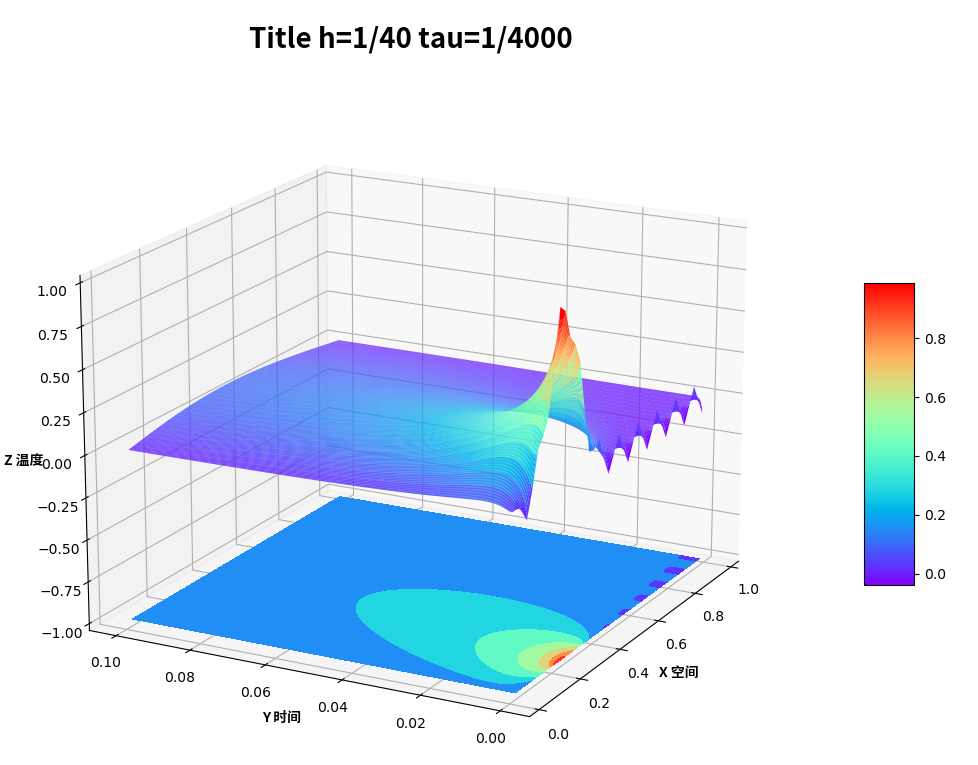
\includegraphics[scale= 0.2]{3.png}
    \end{minipage}    
    \caption{不同剖分下的两个图形}
\end{figure}

\section{结果分析}

\subsection{截断误差分析}

\begin{equation}
\ \left \{
\begin{aligned}
R_j^k(u) ={}& \dfrac{u(x_j,t_{k+1})-u(x_j,t_k)}{\tau}-  \\
& \dfrac{u(x_{j+1},t_{k+1})-2u(x_j,t_{k+1})+u(x_{j-1},t_{k+1})}{h^2}
\end{aligned}
\right.
\end{equation}

利用$Taytor$展式,有

\begin{equation}
\ \left \{
\begin{aligned}
\dfrac{u(x_j,t_{k+1})-u(x_j,t_k)}{\tau} &= \dfrac{\partial u}{\partial t}(x_j,t_k)+O(\tau) \\
\dfrac{u(x_{j+1},t_{k+1})-2u(x_j,t_{k+1})+u(x_{j-1},t_{k+1})}{h^2}&=\dfrac{\partial^2 u}{\partial x^2}(x_j,t_{k+1})+O(h^2) \\
&=\dfrac{\partial^2 u}{\partial x^2}(x_j,t_k)+O(\tau)+O(h^2) 
\end{aligned}
\right.
\end{equation}

根据$(14)$式可知,向后差分的截断误差为:

\begin{equation}
R_j^k(u) = O(\tau+h^2)
\end{equation}

\subsection{适定性分析}

适定性分析就是分析线性方程组$(9)$的解是否存在,存在的画解是否是唯一的,先分析矩阵$A$的具有如下的性质

$\blacksquare$ $A$为稀疏矩阵:每行最多只有3个非零元素

$\blacksquare$ $A$的对角元素全是正的,非对角元素是非正的

$\blacksquare$ $A$对角占优性:即对角线元素之和满足大于等于零

根据这些性质,便可以知道矩阵$A$对称正定,可以得到线性方程组$(9)$一定有解,此外,在高等代数中可以知道$(9)$存在唯一解的充分必要条件是它对应的其次方程组只有零解,事实上,由极值原理可知,此时$AU^{k+1} \leq 0$,所以在边界的取值大于内点,故:

\[U_i^{k+1} \leq 0,~~~ i = 1,2,\cdots,N-1\]

同理可得$AU^{k+1} \geq 0$,所以边界的取值小于内点的取值,故:

\[U_i^{k+1} \geq 0,~~~i =1,2,\cdots,N-1\]

因此上式$(9)$的解存在且唯一.

\subsection{稳定性分析}

所谓稳定性,对于抛物型的方程来讲是基于初值稳定,比如当初值条件发生变化后,得到的数值解是否也只是发生很小的变化,通过理论分析可以知道向后差分格式是无条件稳定的,也就是说我们的初值任意取,对时间和空间的剖分也可以任意的剖分,边界条件也可以发生变化,但是得到的结果仍然是可信的.

\subsection{收敛性分析}

由于方程是适定性,差分格式又是稳定的,所以存在一个算子$L$使得

\begin{equation}
L\left| u_j^k - u(x_j,t_k) \right| \leq MR_j^k(u)
\end{equation}

成立,其中$M$为一个与剖分及算子$L$无关的常数

因为截断误差是趋于零的,因此容易知道当剖分足够的小那么数值解就一定会逼近真解.所以是收敛的

\section{附录}

主程序代码\footnote{本次实验报告的代码编程语言为:python,版本:3.8.6,IDE是pytharm 20.3.3 for linux,操作系统基于linux-ubuntu20.10}

\begin{python}
import xt_pde_matrix as matrix
import xt_pde_tools as tools
import numpy as np
import matplotlib.pyplot as plt
from matplotlib import cm
import matplotlib
"""
向后差分格式求解一维抛物方程代码
"""
e = np.e
pi = np.pi
n = int(input("请输入x轴方向的想要划分的内节点数: "))
times = 3000;
tol = 10 ** (-4)
h = 1.0 / (n + 1)
t = int(input("请输入时间轴方向的想要划分的内部层数: "))
tau = 0.1 / (t + 1)
A = np.zeros((n, n))
data = np.zeros(3 * n - 2)
# 考虑到数组不能够用于数组内部,即x[indices[i]],尽管indices[i]是一个数字,看起来似乎可行,
# 但是当indices[i]是一个数组类型时,将是非法的,indices[i]是列表类型时认为合法
indices = []
indptr = [0]  # 有一个0是因为和算法关系,先初始第一个数
u0 = np.zeros(n)
u1 = np.zeros(n)
# err = np.zeros(times)
B = np.zeros((t + 2, n))
r = tau / (h ** 2)

hx = 0
for i in range(n):
    hx = (i + 1) * h
    u0[i] = e ** (-100 * (hx - 0.25) ** 2) + 0.1 * np.sin(20 * pi * hx)

matrix.back_diff(A, n, r)
matrix.csrmatrix(A, data, indices, indptr)
for i in range(n):
    B[0][i] = u0[i]

for i in range(t + 1):
    tools.csrjacobi(data, indices, indptr, u1, u0, times, tol)
    for k in range(n):
        u0[k] = u1[k]
        B[i + 1][k] = u0[k]

# 画数值解图
fig, ax = plt.subplots(subplot_kw={"projection": "3d"})
# Make data.
X = np.arange(h, 1, h)
Y = np.arange(0, 0.1 + tau, tau)
X, Y = np.meshgrid(X, Y)
R = X ** 0 + Y ** 0 - 2
Z = R + B

surf = ax.plot_surface(X, Y, Z, rstride=1, cstride=1, cmap=cm.rainbow)
fig.colorbar(surf, shrink=0.4, aspect=6)
ax.set_zlim(-1, 1)
ax.contourf(X, Y, Z, zdir='z', offset=-1, cmap=cm.rainbow)
zhfont1 = matplotlib.font_manager.FontProperties\
    (fname="/home/xt/PycharmProjects/python_chinese/SourceHanSansSC-Bold.otf")
# 加标题和轴标签,使用:fontsize=20(any number)可以改变标签字体大小
ax.set_xlabel('X 空间', fontproperties=zhfont1)
ax.set_ylabel('Y 时间', fontproperties=zhfont1)
ax.set_zlabel('Z 温度', fontproperties=zhfont1)
ax.set_title("Title h=1/60 tau=1/600", fontproperties=zhfont1, fontsize=20)
plt.show()
\end{python}

调用的函数代码

xt-pde-martix.py

\begin{python}
# 向前差分格式矩阵
def back_diff(A, n, r):
    for i in range(n):
        if i == 0:
            A[i][i] = 2 * r + 1
            A[i][i + 1] = -r
        elif i == n - 1:
            A[i][i] = 2 * r + 1
            A[i][i - 1] = -r
        else:
            A[i][i] = 2 * r + 1
            A[i][i + 1] = -r
            A[i][i - 1] = -r
            
def csrmatrix(A, data, indices, indptr):
    k = 0
    nr = A.shape[0]
    nc = A.shape[1]
    for i in range(nr):
        for j in range(nc):
            if A[i][j] != 0:
                data[k] = A[i][j]
                indices.append(j)
                k += 1
        indptr.append(k)
\end{python}

xt-pde-tools.py

\begin{python}
def csrjacobi(data, indices, indptr,  x, b, times, tol):
    """
    采用压缩矩阵法求解矩阵与向量的乘法,这样当程序运算量较大时候可以节省很多时间
    :param data: 存储矩阵的非零元素
    :param indices: 存储data中元素对应在矩阵的列数
    :param indptr: 存储矩阵中一行的元素在data中的起始位置
    :param x: 需要迭代求解的向量
    :param b: 一个向量
    :param times:迭代的次数
    :param tol: 迭代的精度,采用的是向量的 2-norm 进行计算的
    :return: x 求解的结果, list_times 迭代的次数,
    list_err_norm 迭代的范数误差, err 真解与数值解的误差向量
    """
    size = len(x)
    x1 = np.zeros(size)
    list_times = []  # 用于记录迭代了多少次并返回,方便主函数实现画图
    list_err_norm = []  # 用于记录每次迭代后的范数误差,方便画图
    for i in range(times):  # 控制迭代次数
        for j in range(size):
            x1[j] = b[j]
            for k in range(indptr[j],indptr[j+1]):
                if indices[k] == j:
                    d = data[k]
                else:
                    x1[j] = x1[j] - data[k]*x[indices[k]]
            x1[j] = x1[j] / d
        for j in range(size):
            x[j] = x1[j]  # 完成一次更新替换
        err = np.zeros(size)
        for k in range(size):
            for j in range(indptr[k],indptr[k+1]):
                err[k] += data[j]*x[indices[j]]
            err[k] = b[k] - err[k]
        err_norm = np.linalg.norm(err)  # 2-norm
        list_times.append(i)
        list_err_norm.append(err_norm)
        # print(err_norm)
        if err_norm < tol:
            break
    return x, list_times, list_err_norm, err
\end{python}

\end{document}